\documentclass{article}
\usepackage{arxiv}

\usepackage[utf8]{inputenc}
\usepackage[english]{babel}
\usepackage[T1]{fontenc}
\usepackage{url}
\usepackage{booktabs}
\usepackage{amsfonts}
\usepackage{nicefrac}
\usepackage{microtype}
\usepackage{lipsum}
\usepackage{graphicx}
\usepackage{natbib}
\usepackage{doi}
\usepackage{amsmath}



\title{Mitigating distributional biases in contrastive learning}

\author{ Lidia Troeshestova \\
	Moscow Institute of Physics and Technology\\
	\texttt{troeshestova.ls@phystech.edu} \\
	%% examples of more authors
	\And
	Roman Isachenko\thanks{Use footnote for providing further information about author (webpage, alternative address)---\emph{not} for acknowledging funding agencies.} \\
	   \\
	\texttt{} \\
	%% \AND
	%% Coauthor \\
	%% Affiliation \\
	%% Address \\
	%% \texttt{email} \\
	%% \And
	%% Coauthor \\
	%% Affiliation \\
	%% Address \\
	%% \texttt{email} \\
	%% \And
	%% Coauthor \\
	%% Affiliation \\
	%% Address \\
	%% \texttt{email} \\
}
\date{}

\renewcommand{\shorttitle}{\textit{arXiv} Template}

%%% Add PDF metadata to help others organize their library
%%% Once the PDF is generated, you can check the metadata with
%%% $ pdfinfo template.pdf
\hypersetup{
pdftitle={A template for the arxiv style},
pdfsubject={q-bio.NC, q-bio.QM},
pdfauthor={David S.~Hippocampus, Elias D.~Striatum},
pdfkeywords={First keyword, Second keyword, More},
}

\begin{document}
\maketitle

\begin{abstract}
	Recently there has been a renewed interest in using contrastive learning for self-supervised representation learning. A popular method for learning representations without labels is to compare similar (positive) and dissimilar (negative) pairs of samples. However, negative samples are often chosen randomly, which means that they could be of the same class. This paper analyzes various ways to eliminate these biases. Based on the fully-supervised case, we develop debiased contrastive models that account for same-label datapoints without requiring knowledge of true labels, and explore their properties. The experiments are performed on MNIST and CIFAR10 datasets. This will further improve availability of accurate models for classification in tasks where extensive labeling is expensive or inaccessible.
\end{abstract}


\keywords{: Contrastive learning \and Representation learning \and Self-supervised learning}

\section{Introduction}
Representation learning has become increasingly popular in recent years due to its ability to learn meaningful representations from large amounts of data, without the need for manual feature engineering. A widely used solution for this problem is contrastive learning, a technique that uses the principle of contrasting samples against each other to learn attributes that are common between data classes and attributes that set apart a data class from another. It encourages the representations of similar pairs $(x, x^+)$ to be close, and those of dissimilar pairs $(x, x^-)$ to be more orthogonal.

The basic metric for supervised similarity is \textit{triplet loss} \citep{schroff2015facenet}, where \textbf{x} is called \textit{anchor}, \textbf{x}$^+$ is a sample with the same label as anchor, and \textbf{x}$^-$ is a sample with the different label than anchor. An improvement of triplet loss is \textit{Multi-class N-pair Loss} invented by \citep{NIPS2016_6b180037}:

\begin{equation} \label{eq:1}
\mathcal{L}(\textbf{x}, \textbf{x}^+, \{\textbf{x}_i^-\}_{i=1}^{N-1}; f) = - \log \frac{\exp(f^T f_i^+)}{\exp(f^T f_i^+) + \sum _{i=1}^{N-1} \exp(f^Tf_i^-)}
\end{equation}

Contrastive learning has proven to be effective for eliciting visual representations: SimCLR  \citep{Chen2020SimCLR} is a framework that considerably outperforms previous self-supervised and semi-supervised learning methods. Its authors developed NT-Xent loss (normalized temperature-scaled cross entropy loss), that uses cosine similarity instead of scalar products.

Due to the unavailability of actual labels during training, negative instances $x^-$ are often randomly selected from the training data. However, this approach results in sampling bias, where $x^-$ may actually be similar to $x$. This bias causes a significant drop in performance. 

To address this issue, \citep{khosla2021supervised} extend the self-supervised batch contrastive approach to the fully-supervised setting, allowing to effectively leverage label information. According to the experiments, supervised contrastive loss outperforms the base cross entropy, but only by a small amount. It also outperforms the cross entropy on robustness benchmark (ImageNet-C, which applies common naturally occuring perturbations such as noise, blur and contrast changes to the ImageNet dataset) and is less sensitive to hyperparameter changes.

As for the case of self-supervised learning, a debiased contrastive loss was proposed to mitigate the bias of negative sampling by \citep{chuang2021debiased}. Given $N$ negative and $M$ positive samples, $\mathcal{L}^{N, M}_{\text{Debiased}} (f)$ is the loss function that corrects for False Negative samples. To remain unsupervised in practice, samples are acquired from the data distribution and a positive distribution mimicked by data augmentations, which can contatin False Positives.

This work aims to develop a new algorithm for debiased sampling in contrastive learning, which accounts for False Positive as well as False Negative samples. In addition, it is suggested to tackle the issue of choosing a wrong anchor in multimodal applications such as attribute detection.



\section{Problem Statement}
\label{sec:headings}

\subsection{Debiased Contrastive Learning}

In \citep{chuang2021debiased} the distribution over classes is denoted by $\rho(c)$, the joint distribution $p_{x,c}(x, c) = p(x|c)\rho(c)$. Let $h : X \rightarrow C$ be the function assigning the latent class labels. Then $p^+_x(x') = p(x'|h(x') = h(x))$ is the probability of observing $x'$ as a positive example for x and $p^-_x(x') = p(x'|h(x') \neq h(x))$ the probability of a negative example. It is assumed that the class probabilities $\rho(x) = \tau^+$ are uniform, and $\tau^- = 1 - \tau^+$ is the probability of observing any different class. Then the  ``ideal``, or unbiased loss to optimize would be:

\begin{equation}
L_{\text{Unbiased}}^N(f) = \mathbb{E}_{\substack{x \sim p, x^+ \sim p^+_x,\\ x_i^- \sim p_x^-}} \bigg[-\log \frac{e^{f(x)^T f(x^+)}}{e^{f(x)^T f(x^+)} + \sum _{i=1}^N e^{f(x)^T f(x_i^-)}}\bigg]
\end{equation}

In practice, $p_x^-(x_i^-)$ is unavailable.
Thus, the standard solution is to sample negative examples $x_i^-$ from the unlabeled $p(x)$ instead. When drawn from $p(x)$, the sample $x_i^-$ will be of the same class as x with probability $\tau^+$.

\begin{equation}
L_{\text{Biased}}^N(f) = \mathbb{E}_{\substack{x \sim p, x^+ \sim p^+_x,\\ x_i^- \sim p_x}} \bigg[-\log \frac{e^{f(x)^T f(x^+)}}{e^{f(x)^T f(x^+)} + \sum _{i=1}^N e^{f(x)^T f(x_i^-)}}\bigg]
\end{equation}

\paragraph{\underline{Problem statement:}} Derive a loss function that approximates the ideal $L_{\text{Unbiased}}^N$, only having access to $M$ positive samples and samples from the distribution $p$.



The data distribution can be decomposed:
\begin{equation}
p(x') = \tau^+ p^+_x(x') + \tau^-p_x^-(x')
\end{equation}

And the missing $p^-_x(x')$ is derived as
\begin{equation} \label{eq:5}
p_x^-(x') = \frac{p(x') - \tau^+ p^+_x(x')}{\tau^-}
\end{equation}
However, estimating $p(x')$ and $p^+_x(x')$ empirically is computationally expensive, and the authors propose a cheaper way to estimate $p^-_x(x')$, using $N$ samples $\{u_i\}_{i=1}^N$ from $p$ and $M$ samples $\{v_i\}_{i=1}^M$ from $p_x^+$:

\begin{equation} \label{eq:6}
L_{\text{Debiased}}^{N, M} (f) = \mathbb{E}_{\substack{x \sim p; x_+ \sim p_x^+,\\ \{u_i\}_{i=1}^N \sim p^N \\ \{v_i\}_{i=1}^N \sim p_x^+^M}}  \bigg[ -\log \frac{e^{f(x)^T} f(x^+)}{e^{f(x)^T f(x^+)} + N g\big(x, \{u_i\}_{i=1}^N, \{v_i\}_{i=1}^M\big)} \bigg],
\end{equation}

where
\begin{equation}
g\big(x, \{u_i\}_{i=1}^N, \{v_i\}_{i=1}^M\big) = \max \bigg\{ \frac{1}{\tau^-}\bigg(\frac{1}{N} \sum \limits_{i=1}^N e^{f(x)^T f(u_i) - \tau^+ \frac{1}{M} \sum \limits_{i=1}^M e^{f(x)^T f(v_i)}}\bigg), e^{-1/t}\bigg\}
\end{equation}

Using this loss on SimCLR framework allowed to achieve higher accuracy compared to the regular biased loss. With a similar theoretical inference, this work is aimed at developing a new algorithm, that would additionally focus on eliminating bias caused by False Positives.

\paragraph{\underline{Tasks:}} 
\begin{itemize}
  \item reproduce Debiased Contrastive Learning results
  \item develop novel debiased contrastive loss that accounts for False Positives.
  \item test the algorithm on CIFAR10 and MNIST datasets
\end{itemize}


\subsection{False Positive Samples}
False Positive samples can be encountered in contrastive learning due to excessive or inappropriate augmentation. Similar to Debiased Contrastive Learning, we propose to estimate the positive sampling distribution in the loss function.
\begin{equation}
p_x^+ (x') = \frac{p(x') - \tau^- p^-_x(x')}{\tau^+}
\end{equation}
Contrary to Debiased Contrastive Learning, drawing samples from $p(x')$ will also include positive labelled datapoints, since some of them could be actually negative. With $N \to \infty$:
\begin{equation}
\mathbb{E}_{\substack{x \sim p \\ x^+ \sim p_x^+ \\ \{x_i^-\}_{i=1}^N \sim p^-^N_x}} \bigg[ - \log \frac{\exp(f^T f^+)}{\exp(f^T f^+) + \sum_{i=1}^N \exp(f^T f_i^-)} \bigg] \longrightarrow \mathbb{E}_{\substack{x \sim p \\ x^- \sim p_x^-}} \bigg[ - \log \frac{R}{R + N \mathbb{E}_{x^- \sim p_x^-} \exp(f^t f^-)} \bigg],
\end{equation}

where
\begin{equation}
R = \frac{1}{\tau^+} (\mathbb{E}_{x' \sim p} \exp(f^Tf') - \tau^- \mathbb{E}_{x^- \sim p_x^-} \exp(f^tf^-))
\end{equation}

With finite N:
\begin{equation} \label{eq:11}
L_{\text{Debiased}}^N (f) = \mathbb{E}_{\substack{x \sim p \\ \{u_i\}_{i=1}^N \sim p^-^N \\ v \sim p_x^+}} \bigg[-\log \frac{R' - \tau^- R^-}{R' + (N \tau^+ - \tau^-) R^-}\bigg],
\end{equation}

where
\begin{equation}
R^-= \frac{1}{N} \sum\limits_{i=1}^N \exp(f(x)^Tf(u_i));
\end{equation}

\begin{equation}
R' = \exp(f(x)^T f(v)) + R^-
\end{equation}

When the number of positive samples $M > 1$, similar to \citep{khosla2021supervised} we will aggregate using the summation over positives located outside of the log (which yields better accuracy for supervised contrastive losses rather than summation inside of the log):
\begin{equation} \label{eq:14}
L_{\text{Debiased}}^{N, M} (f) = \mathbb{E}_{\substack{x \sim p \\ \{u_i\}_{i=1}^N \sim p^-^N \\ \{v_i\}_{i=1}^M}} \frac{1}{M} \sum\limits^M \bigg[-\log \frac{R' - \tau^- R^-}{R' + (N \tau^+ - \tau^-) R^-}\bigg]
\end{equation}

\subsection{Wrong Anchor}
This issue arises in downstream applications of contrastive learning such as image attribute detection, e.g. discrepancy between the image (image representation $f$) and its description (description representation $t$) in online shopping. To solve this problem, when calculating the losses for each picture, we propose to weigh the losses by the cosine similarity of the anchor image vector and the description text vector.

\begin{equation} \label{eq:15}
L_{\text{Unbiased}}(x, x^+, \{x_i^-\}_{i=1}^{N-1}; f) = - \text{sim} (f^T, t^T) \log \frac{\exp(f^T f_i^+)}{\exp(f^T f_i^+ + \sum_{i=1}^N \exp(f^T f_i^-)}
\end{equation}


\section{Experiment}
\subsection{Baseline Reproduction}

The goal of the experiment is to compare Multi-class N-pair Loss \ref{eq:1} with Negative-Debiased Loss \ref{eq:6}. We use STL10 \citep{pmlr-v15-coates11a} dataset, an image recognition dataset for developing unsupervised feature learning algorithms. It contains 100000 unlabeled images of 96x96 pixels for unsupervised learning. The baseline negative-debiased model is SimCLR \citep{Chen2020SimCLR} with ResNet-18 \citep{7780459} as the encoder architecture, with the Adam optimizer \citep{Diederik2014Adam} with learning rate 0.001. All models are trained for 50 epochs and evaluated by training a linear classifier after fixing the learned embedding.

 The results are shown in Figure \ref{fig:fig1}. While the difference between Top-5 accuracy for the debiased model and the biased model is insignificant, Top-1 accuracy of the debiased model is higher than that of the biased model. 

\begin{figure}[!htb]
\minipage{0.49\textwidth}
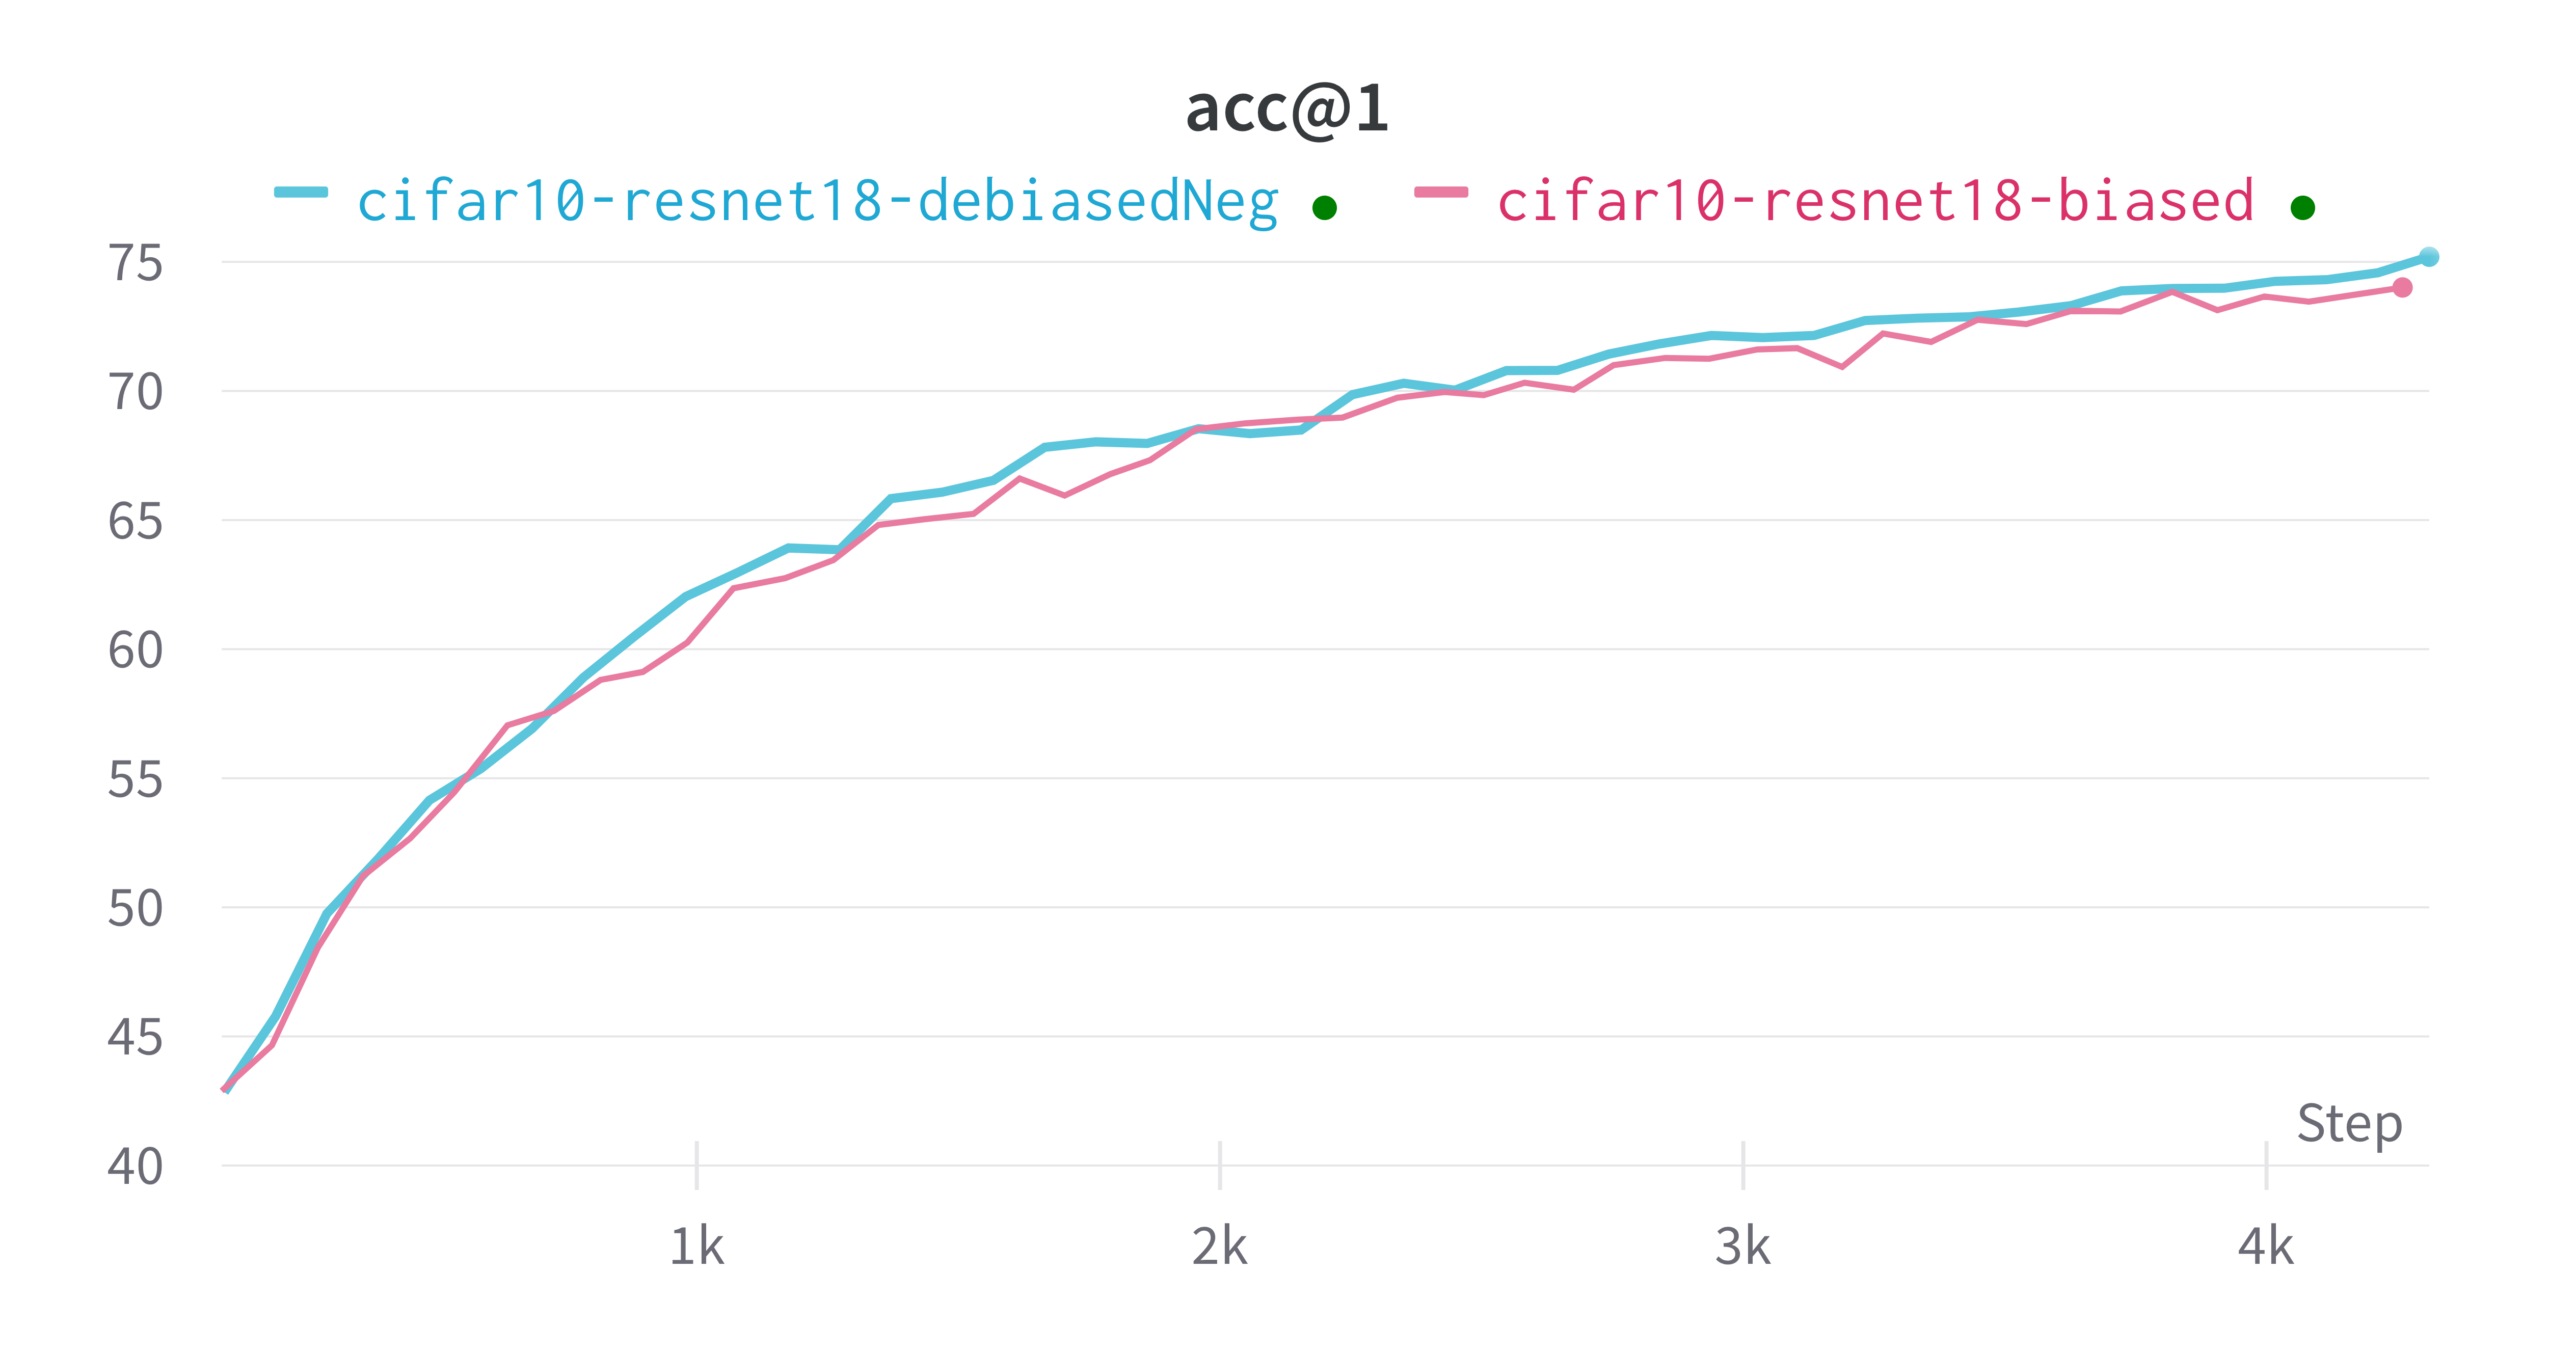
\includegraphics[width=\linewidth]{figures/baseline_acc1.png}
\endminipage\hfill
\minipage{0.49\textwidth}
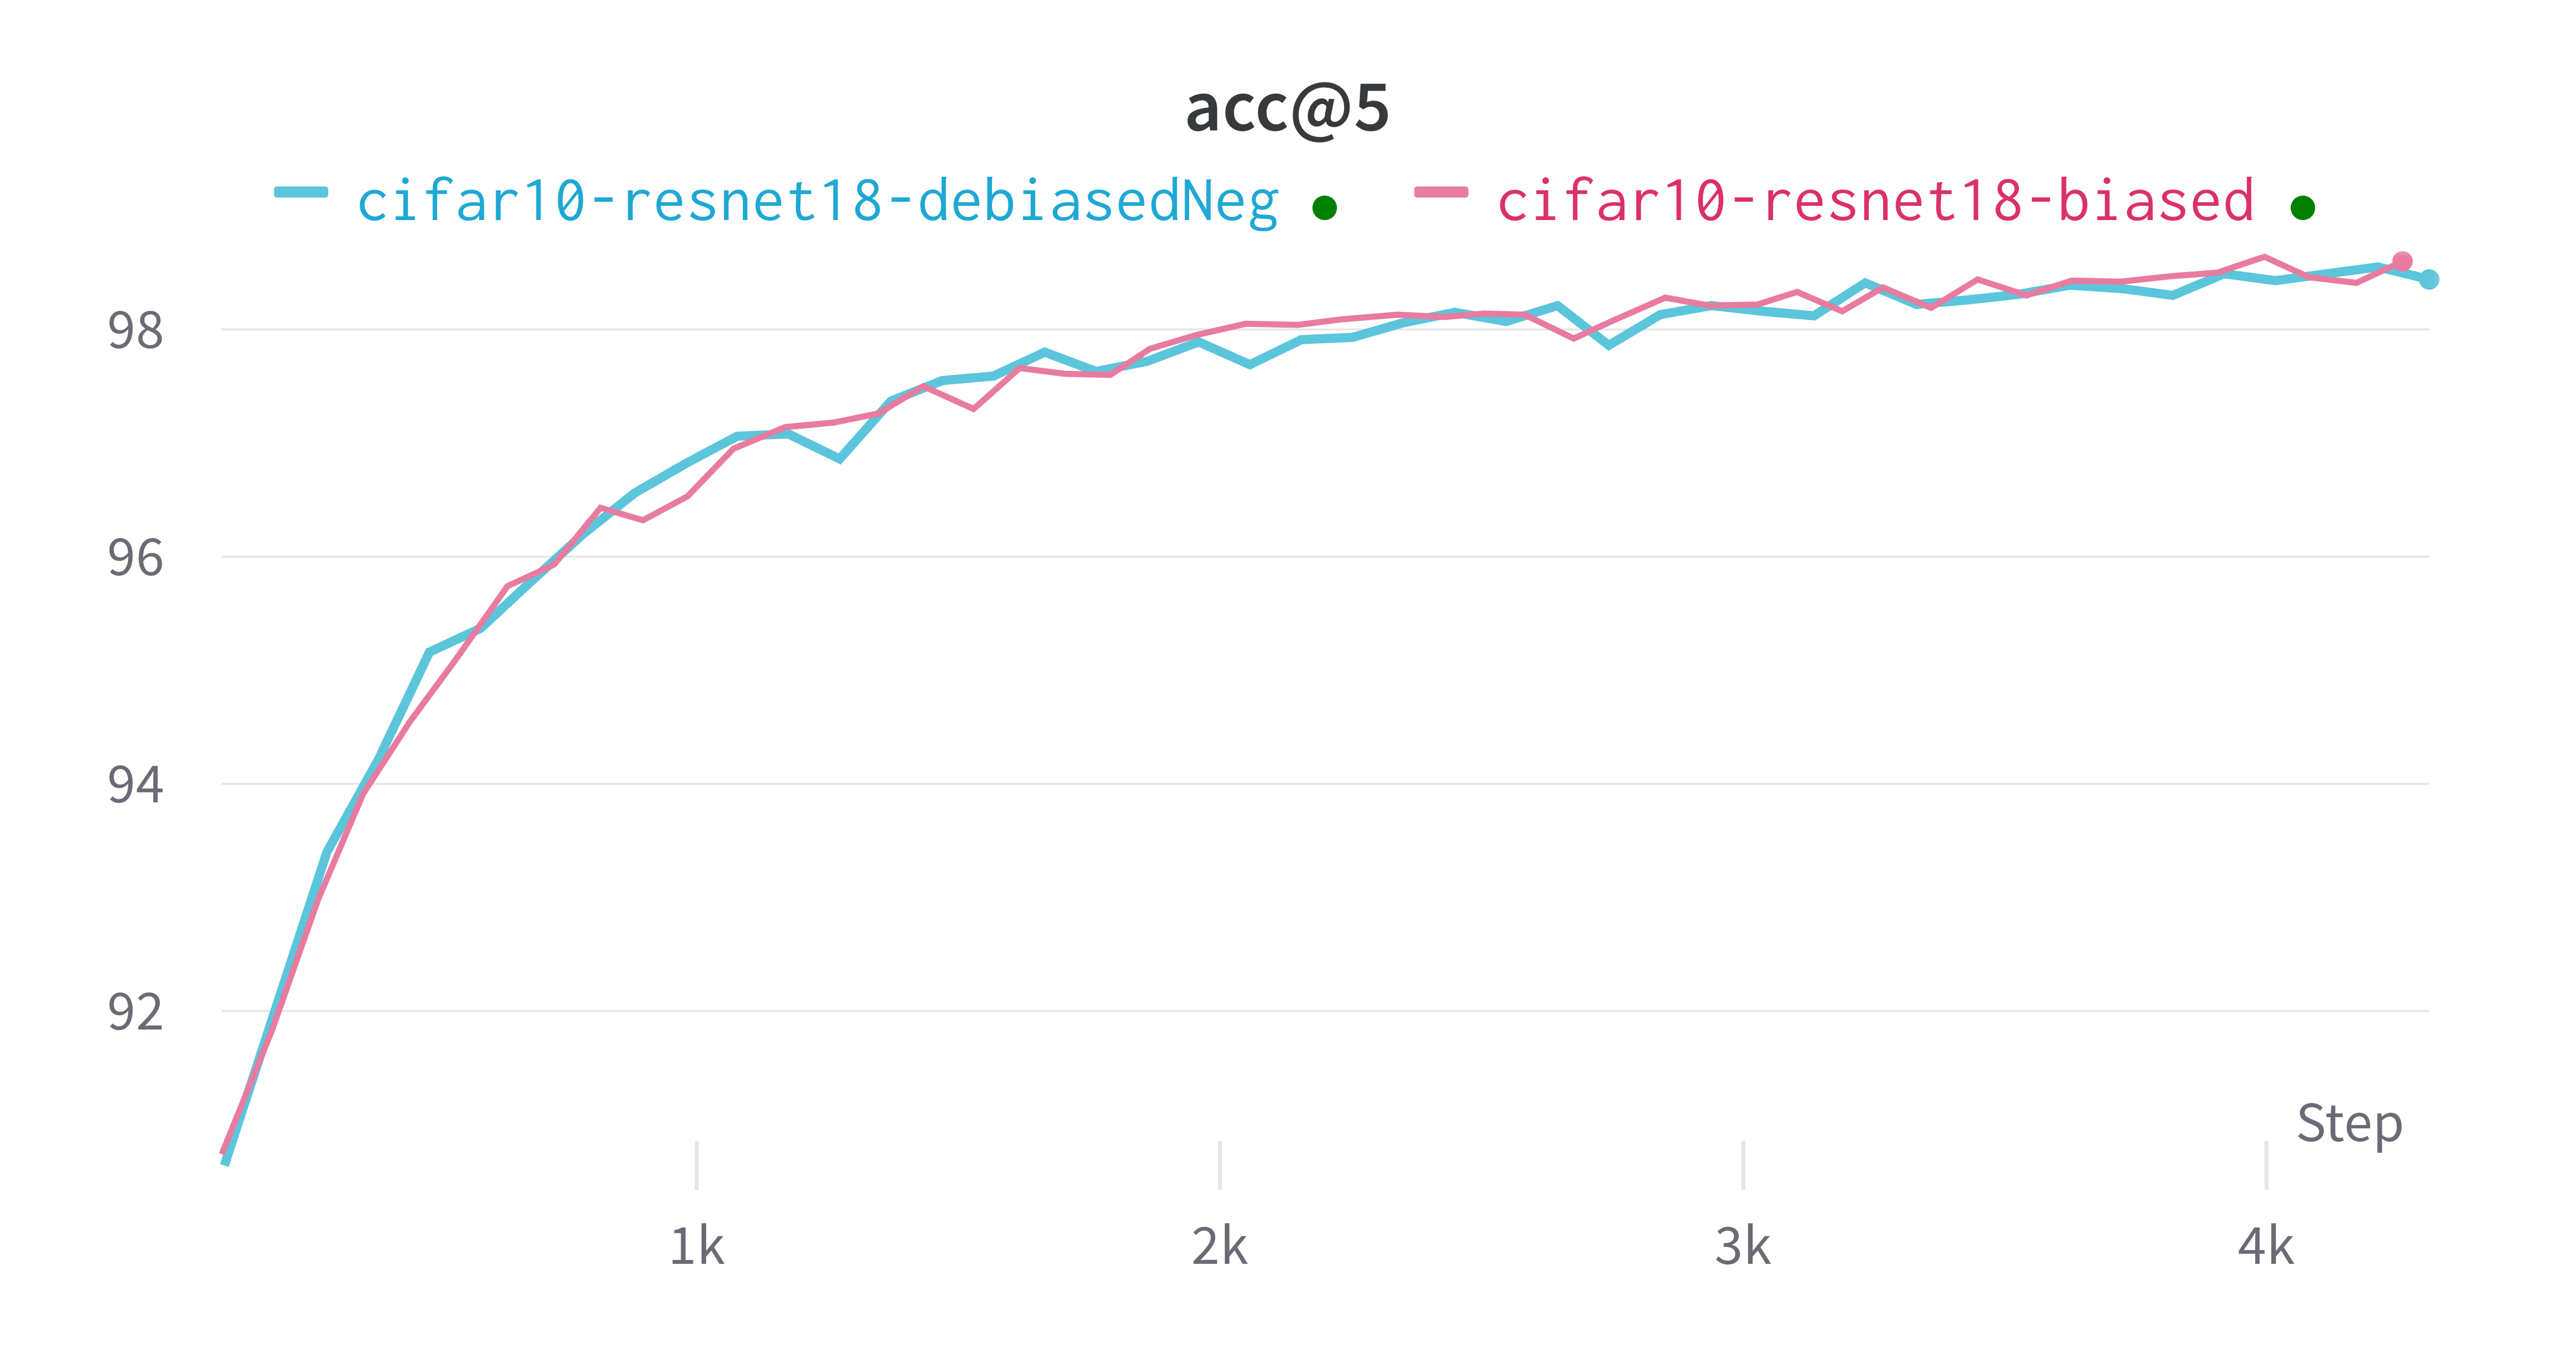
\includegraphics[width=\linewidth]{figures/baseline_acc5.png}
\endminipage
\caption{Classification accuracy on CIFAR10, Biased contrastive loss and Debiased-Neg.}
\label{fig:fig1}
\end{figure}

\subsection{Testing New Loss}
We run the same experiment for Positive-Debiased loss \ref{eq:14}. Figure \ref{fig:fig2} shows a tangible difference between the performances of the novel loss and the previous losses. The accuracy advantage is prevalent from the very first steps of training both for Top-1 and Top-5 accuracy, meaning Positive-Debiased loss is more efficient in the early stages of training.  


% \begin{figure}
% 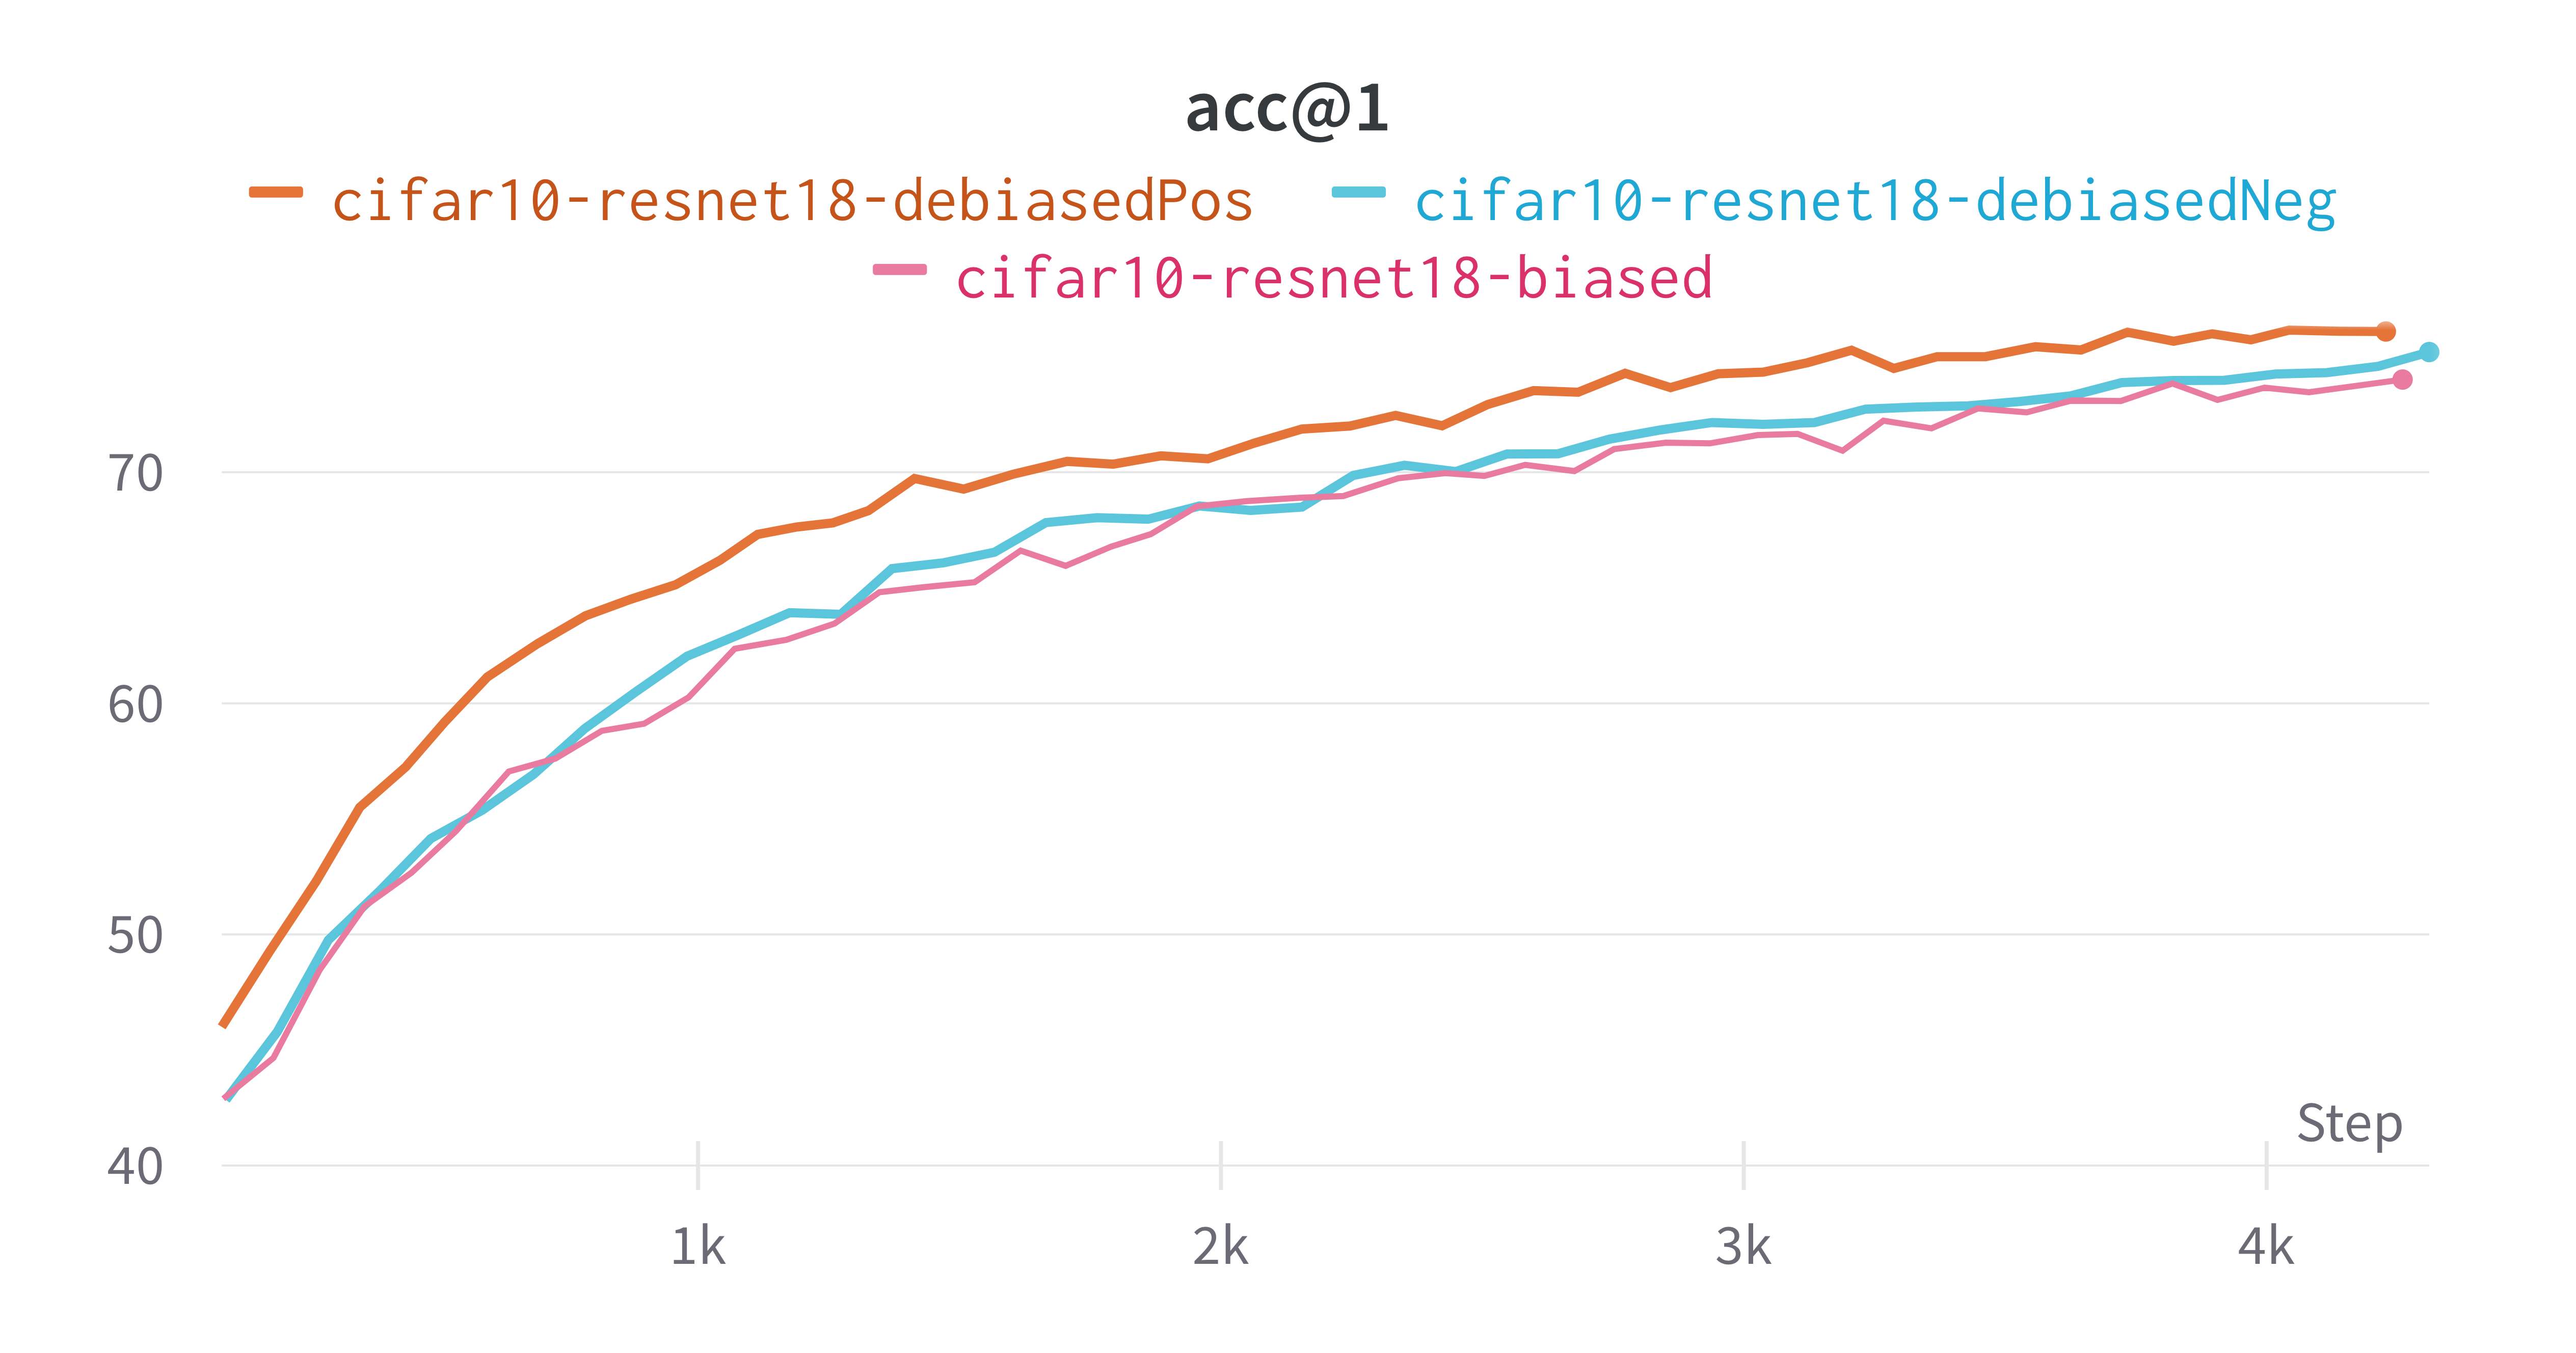
\includegraphics[width=0.5\textwidth]{figures/3_losses.png}
% 	\caption{Loss functions}
% 	\label{fig:fig1}
% \end{figure}

\begin{figure}[!htb]
\minipage{0.49\textwidth}
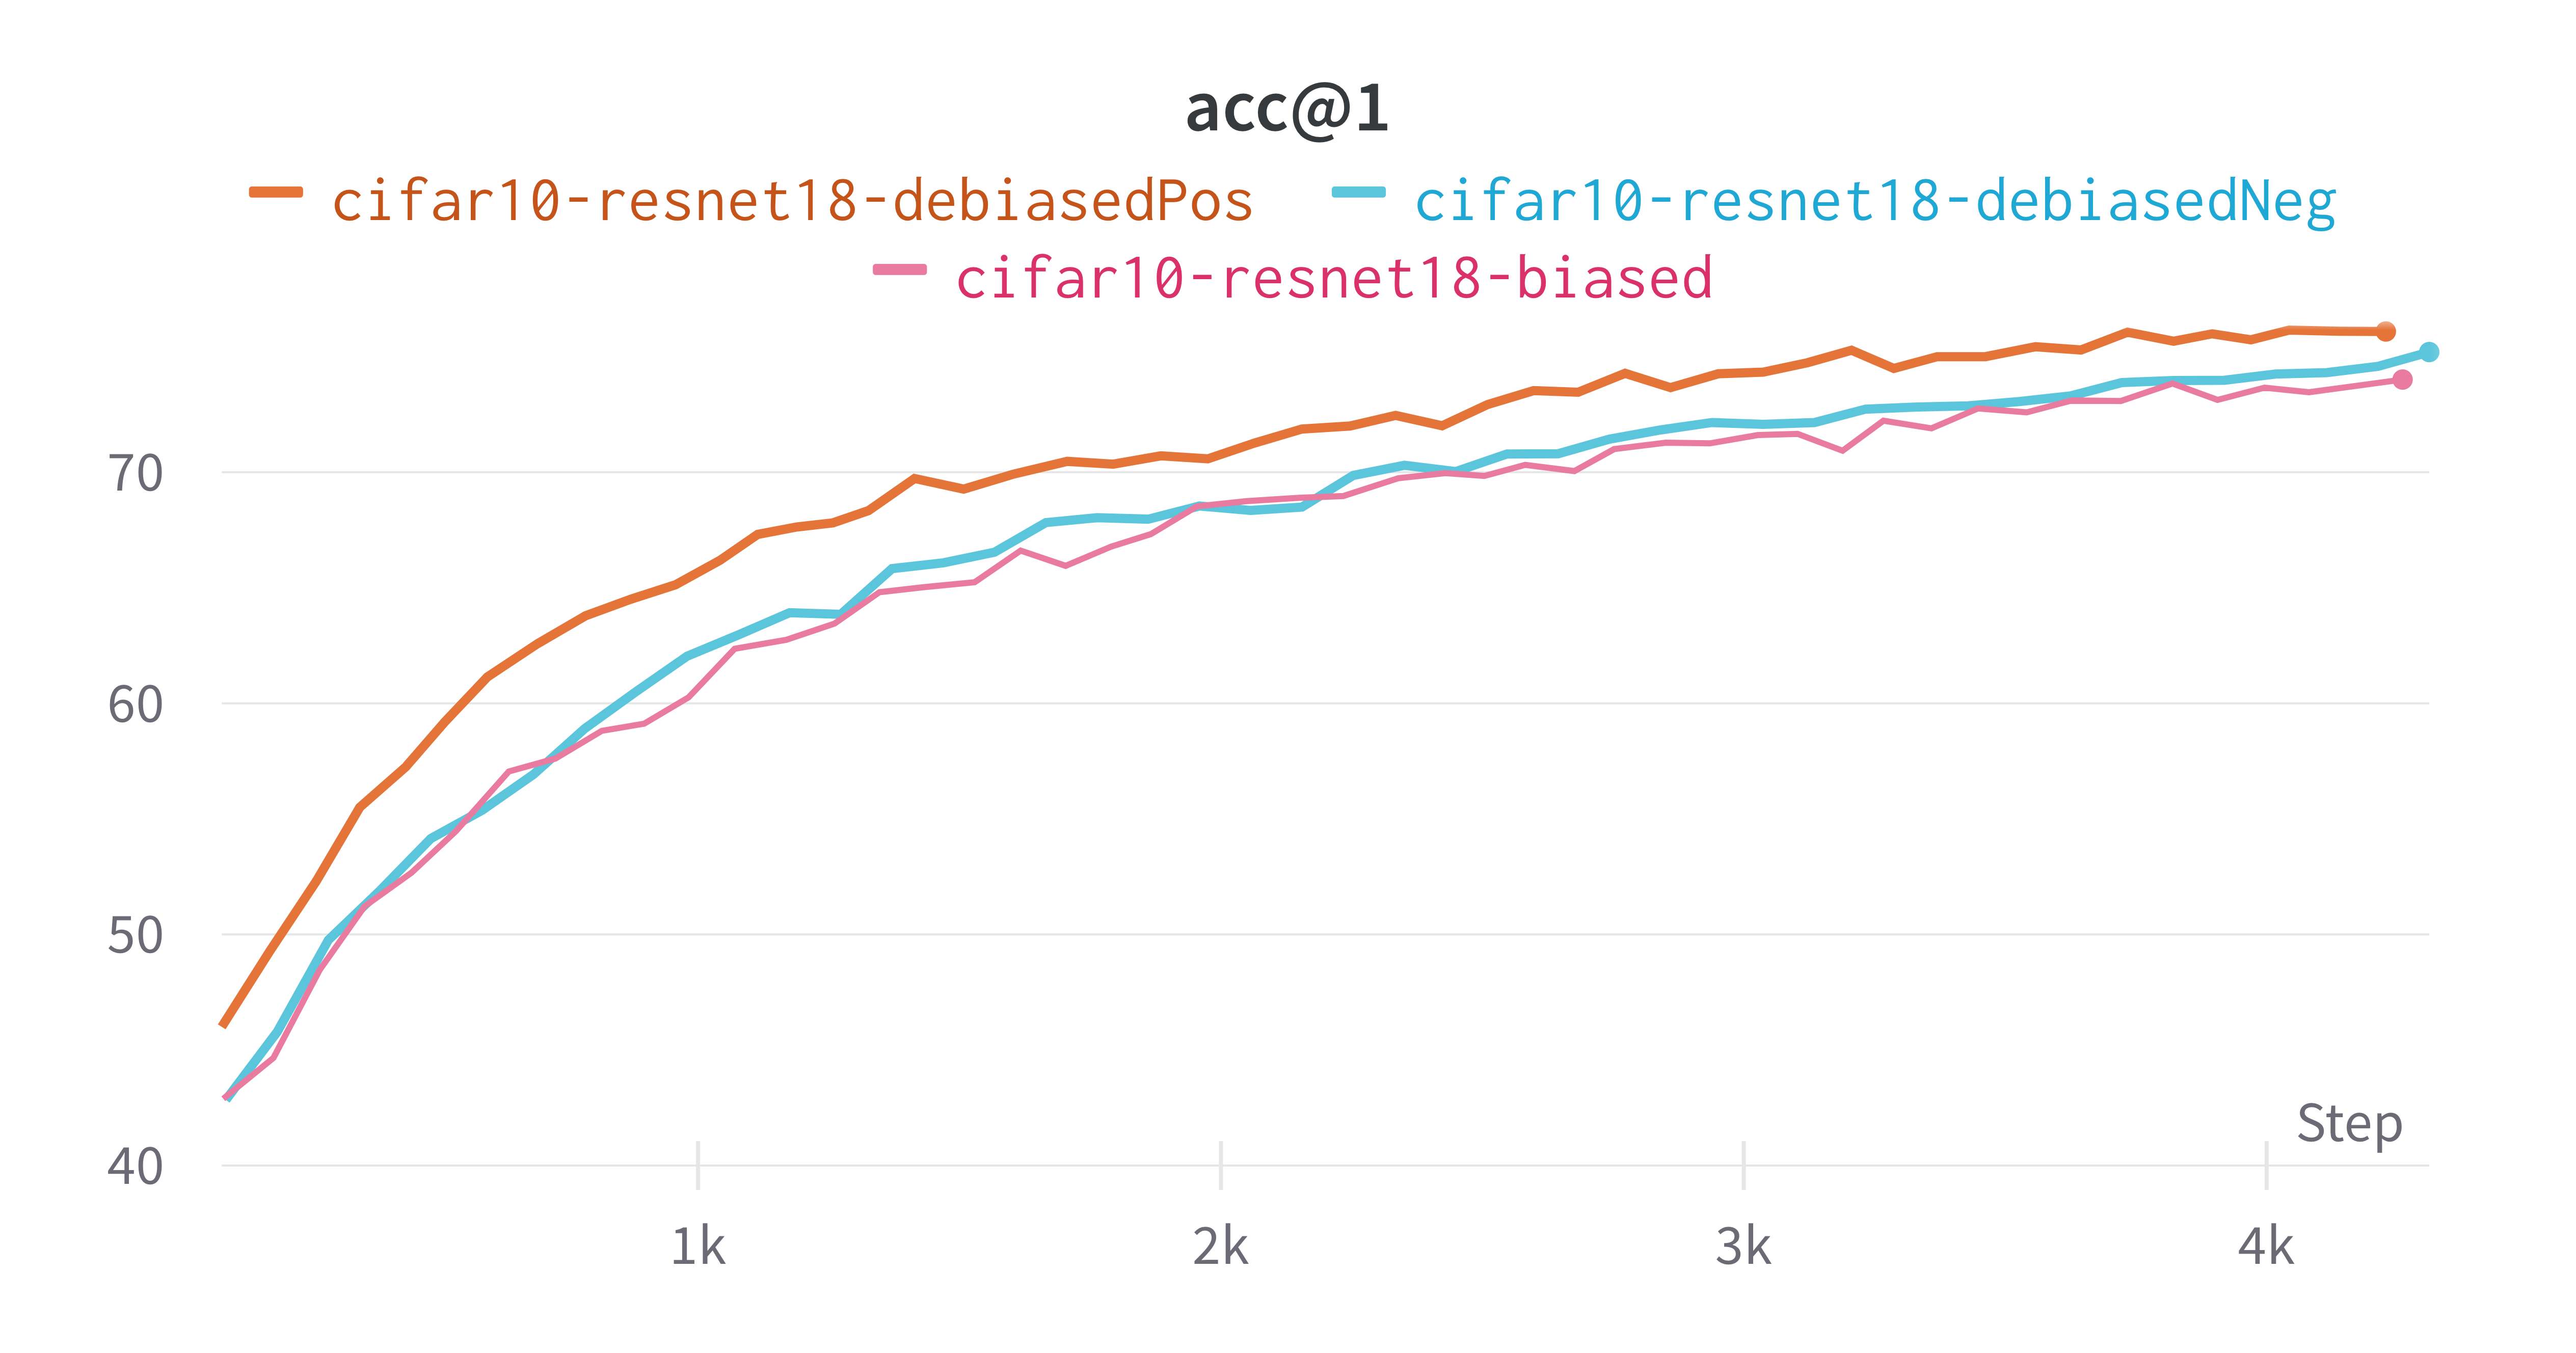
\includegraphics[width=\linewidth]{figures/3_losses.png}
\endminipage\hfill
\minipage{0.49\textwidth}
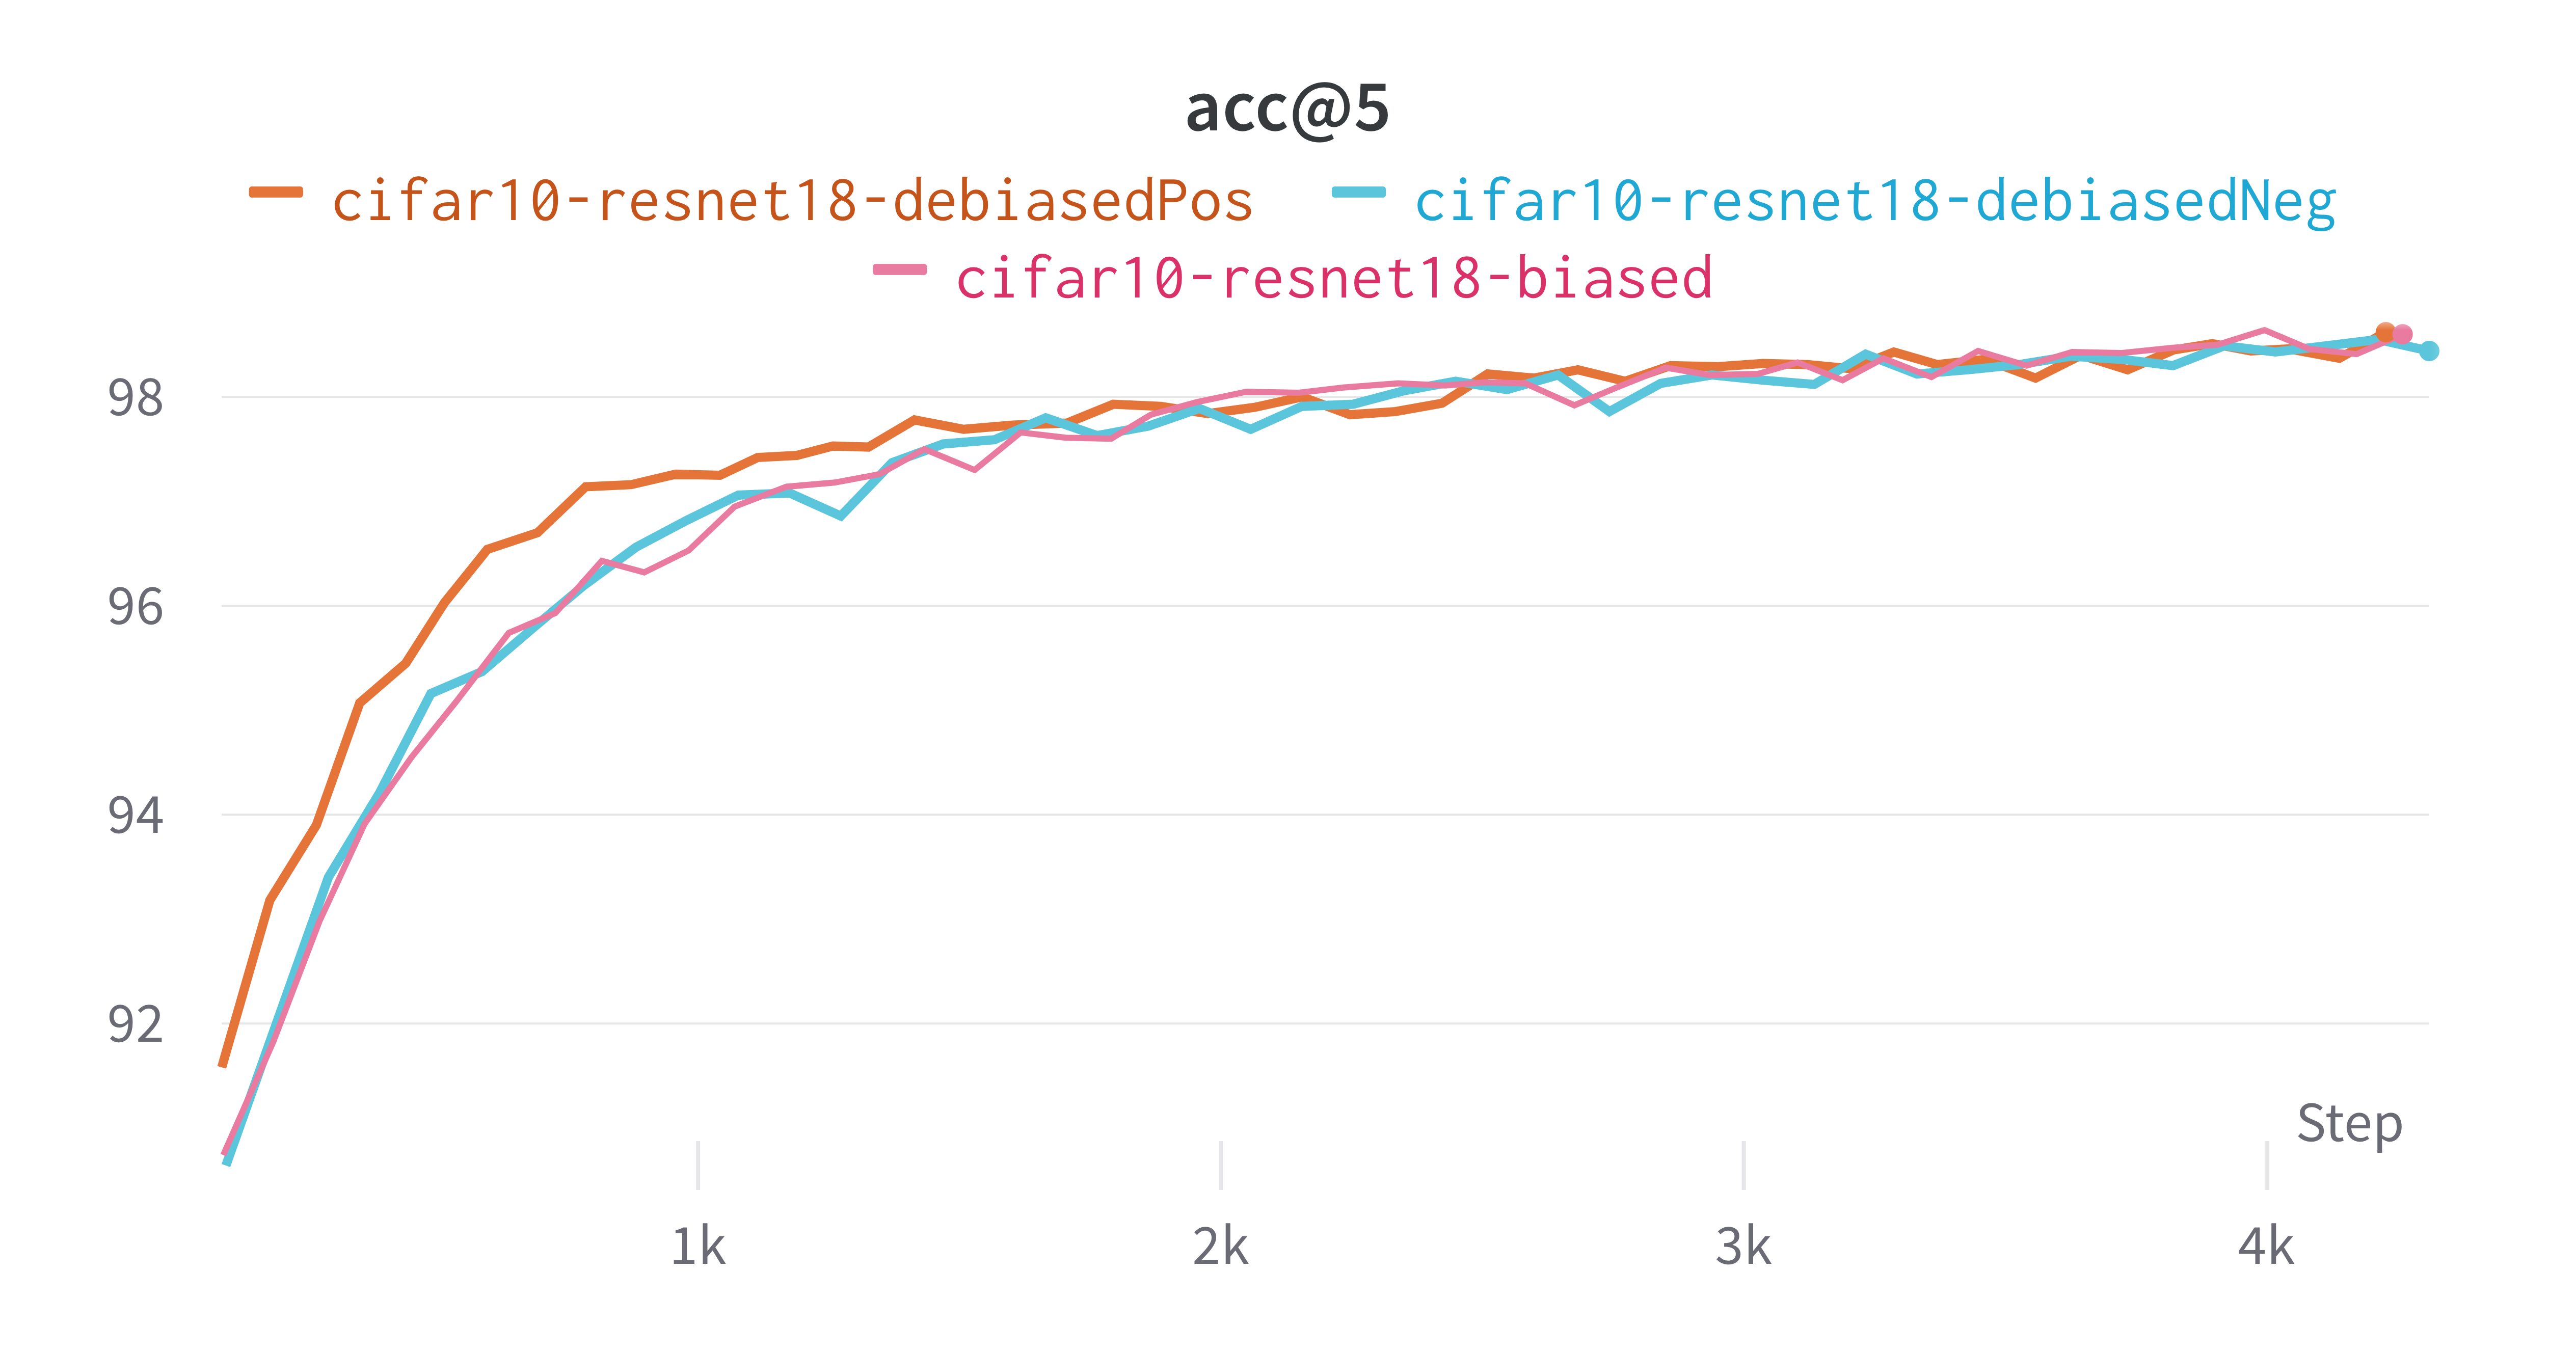
\includegraphics[width=\linewidth]{figures/3_losses_5.png}
\endminipage
\caption{Classification accuracy on CIFAR10, Debiased-Pos.}
\label{fig:fig2}
\end{figure}

\noindent\rule{16cm}{0.4pt}


\section{Examples of citations, figures, tables, references}
\label{sec:others}

\subsection{Citations}
Citations use \verb+natbib+. The documentation may be found at
\begin{center}
	\url{http://mirrors.ctan.org/macros/latex/contrib/natbib/natnotes.pdf}
\end{center}

Here is an example usage of the two main commands (\verb+citet+ and \verb+citep+): Some people thought a thing \citep{kour2014real, hadash2018estimate} but other people thought something else \citep{kour2014fast}. Many people have speculated that if we knew exactly why \citet{kour2014fast} thought this\dots

\subsection{Figures}
\lipsum[10]
See Figure \ref{fig:fig1}. Here is how you add footnotes. \footnote{Sample of the first footnote.}
\lipsum[11]



\subsection{Tables}
See awesome Table~\ref{tab:table}.
See Section \ref{sec:headings}.

The documentation for \verb+booktabs+ (`Publication quality tables in LaTeX') is available from:
\begin{center}
	\url{https://www.ctan.org/pkg/booktabs}
\end{center}




\subsection{Lists}
\begin{itemize}
	\item Lorem ipsum dolor sit amet
	\item consectetur adipiscing elit.
	\item Aliquam dignissim blandit est, in dictum tortor gravida eget. In ac rutrum magna.
\end{itemize}

\begin{table}
	\caption{Sample table title}
	\centering
	\begin{tabular}{lll}
		\toprule
		\multicolumn{2}{c}{Part}                   \\
		\cmidrule(r){1-2}
		Name     & Description     & Size ($\mu$m) \\
		\midrule
		Dendrite & Input terminal  & $\sim$100     \\
		Axon     & Output terminal & $\sim$10      \\
		Soma     & Cell body       & up to $10^6$  \\
		\bottomrule
	\end{tabular}
	\label{tab:table}
\end{table}

\bibliographystyle{unsrtnat}
\bibliography{references}

\end{document}